\documentclass[a4paper, 12pt, french]{article}
%\immediate\write18{texcount -tex -sum -char \rapport.tex > /tmp/wordcount.tex}
\usepackage[utf8]{inputenc}
\usepackage[T1]{fontenc}
\usepackage{babel}
\usepackage{setspace}
\usepackage{hyperref}
\usepackage{imakeidx}
\usepackage{graphicx}
\usepackage{fancyhdr}
\usepackage{chngcntr}
\usepackage{pifont}
\usepackage{xcolor}
\usepackage{glossaries}
\usepackage{helvet}
\usepackage{titlesec}
\usepackage{tikz}
\usepackage{rotating}
\usepackage{lscape}
\usepackage{wrapfig}
\usepackage[stable]{footmisc}
\usepackage{comment}
\usepackage{enumitem}

\makeindex[intoc]
 
\counterwithin{figure}{section}
\counterwithin{table}{section}

\setcounter{tocdepth}{4}
\setcounter{secnumdepth}{4}
\setcounter{tocdepth}{5}
\setcounter{secnumdepth}{5}

\definecolor{ssiYellow}{RGB}{255,237,0}
\definecolor{ssiRed}{RGB}{231,0,14}
\definecolor{ssiBlack}{RGB}{18,18,13}

%\newcommand{\bsquare}{\item[\color{myblue}\ding{110}]} 
%\newcommand{\barrow}{\item[\color{myblue}\ding{228}]}
%\newcommand{\bwarrow}{\item[\color{myblue}\ding{227}]}

\newcommand{\bdot}{\item[\color{ssiYellow}\ding{108}]} 
\newcommand{\bdotoutlined}{\item[\color{ssiYellow}\ding{109}]}
\newcommand{\bsquare}{\item[\color{ssiYellow}\ding{110}]}
\newcommand{\bsquareoutlined}{\item[\color{ssiYellow}\ding{111}]}
\newcommand{\bdiamond}{\item[\color{ssiYellow}\ding{117}]}
\setlistdepth{9}
\renewlist{itemize}{itemize}{9}

%remove red border on links in the table of contents and green border for bibliography ..
%change links style : remove border by making it white
\hypersetup{%
    pdfborder = {0 0 0}
}
\renewcommand{\familydefault}{\sfdefault}

\titleformat{name=\section}{\normalfont\Large\bfseries\color{ssiBlack}}{\color{ssiYellow}\rule[-1.35mm]{3em}{1.25em}{\color{white}\hspace{-1cm}\normalfont\Large\bfseries\thesection\hspace{15pt}}}{1em}{}[\color{ssiYellow}{\titlerule[4pt]}\vspace*{4pt}]
\titleformat{\subsection}{\normalfont\Large\bfseries\color{ssiBlack}}{\color{ssiRed}\rule[-1.35mm]{3em}{1.25em}{\color{white}\hspace{-1.3cm}\normalfont\Large\bfseries\thesubsection\hspace{10pt}}}{1em}{}[\color{ssiYellow}{\titlerule[3pt]}\vspace*{4pt}]
\titleformat{\subsubsection}{\normalfont\Large\bfseries\color{ssiBlack}}{\color{ssiYellow}\rule[-1.35mm]{3em}{1.25em}{\color{white}\hspace{-1.60cm}\normalfont\Large\bfseries\thesubsubsection\hspace{5pt}}}{1em}{}[\color{ssiYellow}{\titlerule[2pt]}\vspace*{4pt}]

\titleformat{name=\section,numberless=true}{\color{ssiBlack}\normalfont\Large\bfseries}{}{0em}{}[\color{ssiYellow}{\titlerule[4pt]}\vspace*{4pt}]
\titleformat{name=\subsection,numberless=true}{\color{ssiBlack}\normalfont\Large\bfseries}{}{0em}{}[\color{ssiYellow}{\titlerule[3pt]}\vspace*{4pt}]
\titleformat{name=\subsubsection,numberless=true}{\color{ssiBlack}\normalfont\Large\bfseries}{}{0em}{}[\color{ssiYellow}{\titlerule[2pt]}\vspace*{4pt}]

\sloppy

\pagestyle{fancy}
\fancyhf{}
\rhead{Informatique et réseaux}
\lhead{PINEAU Anthony}

\makeglossaries

%\newglossaryentry{latex}{name=latex,description={Is a mark up language specially suited for scientific documents}}
%\newglossaryentry{maths}{name=mathematics,description={Mathematics is what mathematicians do}}
%\newglossaryentry{formula}{name=formula,description={A mathematical expression}}
%\newacronym{gcd}{GCD}{Greatest Common Divisor}
%\newacronym{lcm}{LCM}{Least Common Multiple}

\newglossaryentry{WMS}{name=Warehouse Management System,description={ou Système de Gestion d’Entrepôt est un logiciel informatique dédié à l’optimisation de la gestion des stocks au sein des entrepôts.\footnote{\cite{wms}}}}

\newglossaryentry{WCS}{name=Warehouse Control System,description={ou Système de Pilotage des Activités représente un outil d’optimisation du flux logistique. Un système ou logiciel WCS pilote et synchronise les différents des éléments mécanisés ( Robots, pautomates, convoyeurs, dépose étiquettes , balances ….) de l’entrepôt.\footnote{\cite{wcs}}}}

\newacronym{wms}{WMS}{Warehouse Management System}
\newacronym{wcs}{WCS}{Warehouse Control System}

\begin{document}	
	\begin{titlepage}
		\begin{center}

			\tikz[remember picture,overlay] \node[opacity=0.3,inner sep=0pt] at (current page.center){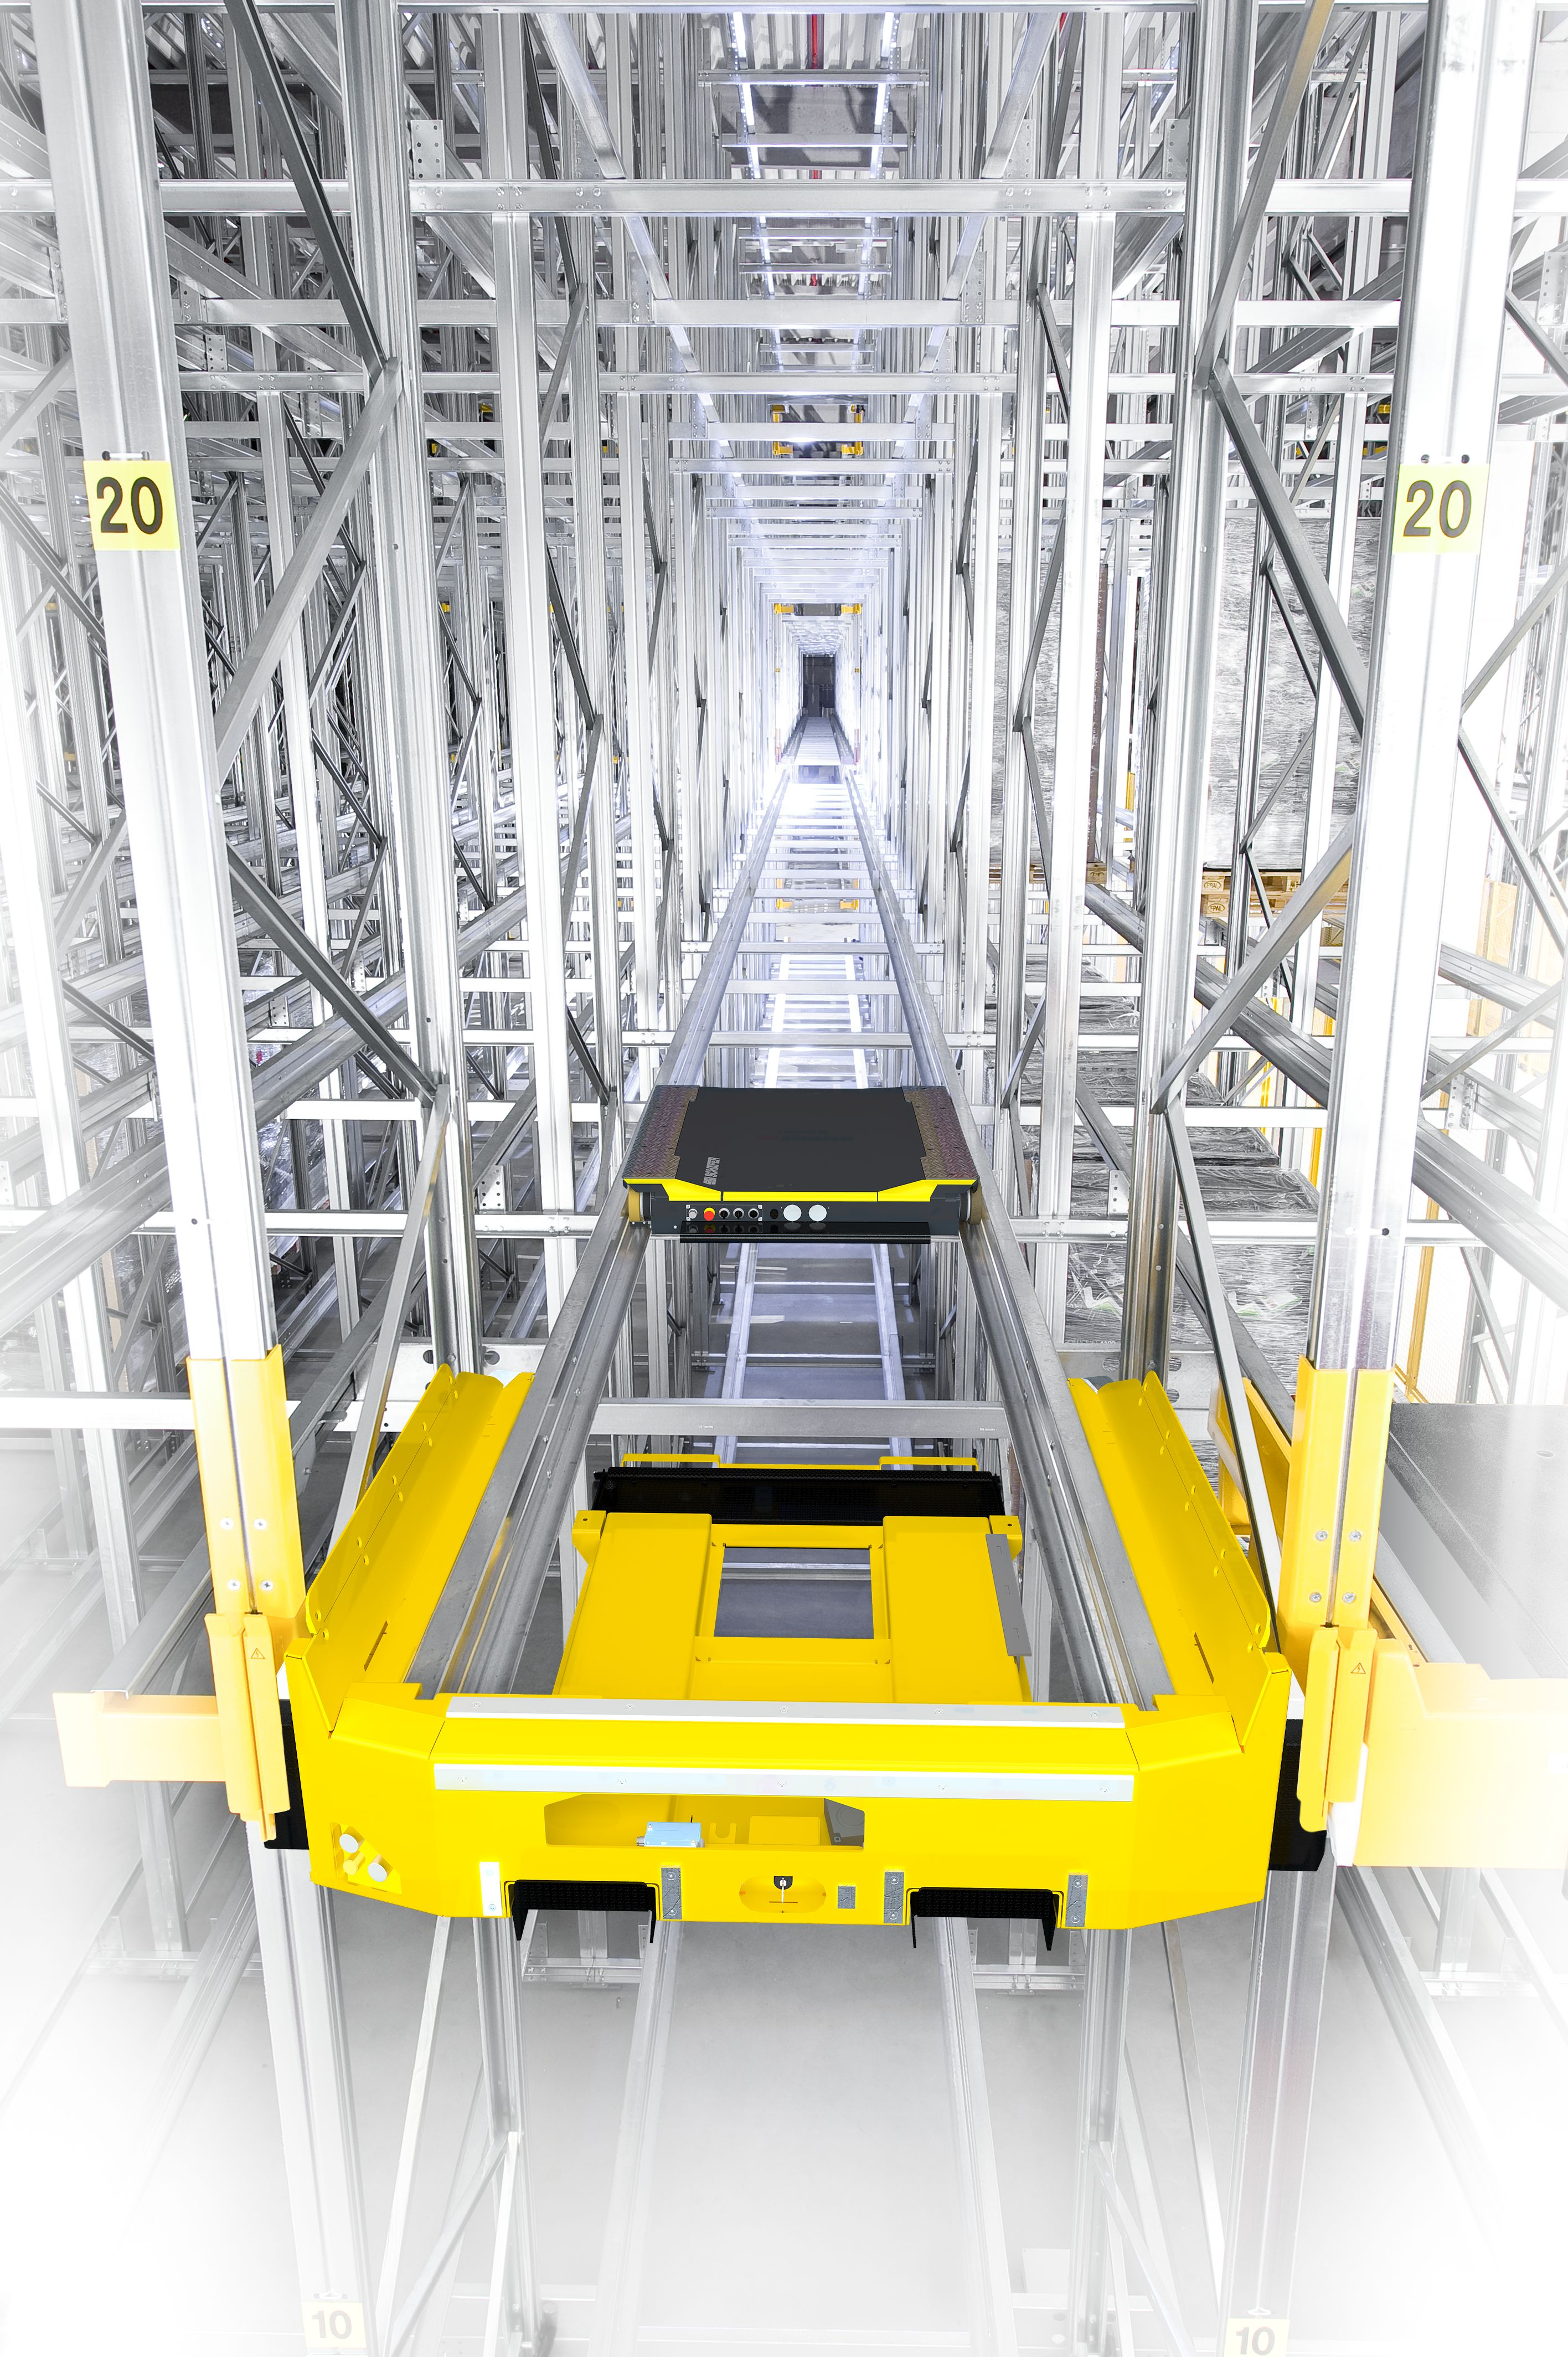
\includegraphics[width=\paperwidth,height=\paperheight]{images/ssi_orbiter_highlight.jpg}};

			%\vspace*{1cm}

			\Huge
			\textbf{Mémoire de fin d'études}

			\vspace{0.5cm}
			\LARGE
			"Comment développer une application web à partir d’un client lourd ?"

			\vspace{1.5cm}

			\textbf{Anthony PINEAU}\\
			\textbf{IR2023}

			\vfill

			
\includegraphics[width=0.6\textwidth]{images/schaefer.jpg}
			\vfill
			
\includegraphics[width=0.4\textwidth]{images/esaip.jpg}

			\vfill

			Stage effectué du\\
			13 mars 2023 au 22 septembre 2023

			\vspace{0.8cm}
			
			\Large
			Maître de stage : Monsieur Thierry NEROT\\
			Tuteur pédagogique : Docteur Sofiane HAMRIOUI\\
		\end{center}
	\end{titlepage}
		
	\newpage

	\footnotesize
	\section*{Remerciements}		
	En premier lieu, je tiens à remercier Monsieur Laurent GOURDON, directeur général France de l'entreprise SSI SCHÄFER, de m’avoir permis de rejoindre à nouveau son équipe et m’avoir offert la possibilité de mettre en pratique mes connaissances et mes compétences acquises pendant mes précédentes années d’études ainsi que ces trois années du cycle ingénieur du numérique à l’ESAIP. \\

	Je tiens ensuite à remercier Monsieur Thierry NEROT, qui, en tant que maître de stage, s'est rendu disponible pour moi, et a su m'accompagner et partager ses connaissances avec moi.\\

	J’en profite pour remercier aussi tous les membres de l’équipe avec qui j’ai pu travailler, Messieurs Sébastien NICOD, Thibaut LUCAS et Pascal MARCELOT, qui ont su se rendre disponible pour moi si besoin. Il a d'ailleurs été très facile pour moi de pouvoir échanger avec eux et j'ai beaucoup appris auprès d'eux.\\

	Par ailleurs, je remercie également tous mes autres collègues qui ont été très accueillants tout au long du stage, Mesdames Charlotte BARGMAN, Océane SACHOT, Pauline CHAPRON, Anita BABONNEAU, Nathalie DELARUE, Roukia ATHOUMANI ainsi que Messieurs Quentin VIOLLEAU, Robin BALLON et Nicolas PERDRIAU.\\

	Je saisis cette occasion pour adresser mes profonds remerciements aux responsables et au personnel de l’ESAIP d’avoir fait le nécessaire en ce qui concerne la gestion des conventions de stage ainsi que de nous soutenir au quotidien dans notre projet pédagogique et professionnel.\\

	Je tiens ainsi à remercier tout particulièrement Monsieur Sofiane HAMRIOUI. En tant que tuteur pédagogique, nous avons pu échanger tout au long de mon stage, parler de l’avancement du projet sur lequel j'ai travaillé ainsi que travailler sur les parties de ce présent mémoire.\\

	Ensuite je tiens à adresser un grand merci à ma famille, sans qui tout cela ne serait pas possible. Merci pour leurs conseils ainsi que leur soutien inconditionnel, à la fois moral et économique. Ils m’accompagnent et me soutiennent au quotidien aussi bien dans mon projet pédagogique que dans mon projet professionnel et sont une source d’inspiration pour moi.\\

	Enfin je tiens à adresser un profond remerciement à ma compagne, Madame Antonia HAMMER, pour son soutien tout au long de mon stage, pour son aide pour la rédaction des parties en allemand de ce présent mémoire ainsi que pour la préparation de la partie allemande de la soutenance. Vielen Dank meine Liebe.

\vspace{\baselineskip}\vspace{\baselineskip}\vspace{\baselineskip}
\noindent
Anthony PINEAU

	\newpage

	\normalsize
	
	\doublespacing
	\tableofcontents

	\vspace{\baselineskip}
	\noindent Nombre de caractères totaux : X caractères\\
	Nombre de caractères en anglais : X caractères\\
	Nombre de caractères en allemand : X caractères\\

	\newpage
		
	\rfoot{Page \thepage}
	
	\phantomsection
	\listoffigures
	\addcontentsline{toc}{section}{\listfigurename}
	
	%\newpage

	\phantomsection
	\listoftables
	\addcontentsline{toc}{section}{\listtablename}
	\newpage

	\phantomsection
	\printglossary
	\addcontentsline{toc}{section}{\glossaryname}

	\newpage
	
	\singlespacing

	\phantomsection
	\section*{Introduction}%à traduire en allemand..
	\addcontentsline{toc}{section}{Introduction}
	De nos jours, les utilisateurs aiment avoir un accès rapide et simple aux logiciels et applications qu’ils utilisent, sans par exemple avoir à installer un client lourd. Ainsi la solution qui s’offre à nous est de leur mettre à disposition une application web.\\

Développer une application web pour faciliter l’accès à l’utilisateur semble une bonne idée mais comment la développer lorsque l’on doit reproduire le comportement d’un client lourd existant ?\\

Ainsi dans le cadre de mon projet de fin d’études, j’ai eu la chance de participer au projet de développement d’une application web issu d’un client lourd qui permettra un déploiement plus rapide ainsi qu’une refonte de l’interface graphique. Cela m’a donc donné l’envie d’approfondir le cheminement du développement d’une application web à partir d’un client lourd.\\

Une application web se compose principalement en deux parties : la partie front-end (interface graphique) et la partie back-end (accès à la base de données, traitement des requêtes). Ainsi notre application sera composée d’une partie interface utilisateur qui fera appel à des requêtes HTTP d’une API REST, qui elle communiquera avec la base de données.\\

Dans ce mémoire, nous nous interrogerons sur le développement d’une application web à partir d’un client lourd, du choix du langage de programmation utilisé (ou framework) au déploiement de l’application en passant par l’implémentation des interfaces graphiques.\\

Afin de traiter le sujet et de répondre aux questionnements émis, un plan de recherche a été établie. Tout d’abord, le choix de langage de programmation a été capital afin de partir sur de bonnes bases. Ensuite le développement d’une nouvelle interface graphique a été mis en place. Pour finir par l’implémentation de la connexion à la base de données au travers d’une API REST.\\

L’objectif est ainsi de comprendre comment développer une application web à partir d’un client lourd et voir quelles sont les principales différences entre les deux solutions.\\

Nous verrons dans un premier temps que le choix du langage de programmation est très important dans le développement d’une application web. Ensuite nous nous intéresserons à la création des interfaces graphiques. Nous devrons également voir la connexion entre l’application web et la base de données via une api REST. Finalement nous verrons le résultat final de l’application avec son déploiement.

	\newpage

	%glossaire
	%\gls{latex}
	%\Glspl{formula} première lettre majuscule et pluriel
	
	%acronyme
	%\acrlong{wms}
	%\acrshort{wms}
	%\acrfull{wms}
	
	%index
	%\index{maths}

	%index + glossaire..
	%\index{\gls{WMS}}

	%à voir index + glossaire + acronyme ..

	%bibliographie
	%\cite{ctan}
	\section{Contexte global\footnote{Références utilisées dans la section \ref{section:context} : \cite{schaefer}, \cite{history}, \cite{schaeferFR}, \cite{schaeferMorpheus}.}}\label{section:context}
		%introduction contexte global
	Afin de bien comprendre les intérêts de ce stage, il est important d'en poser le contexte et notamment de revenir sur l'entreprise SSI SCHÄFER ainsi que la suite de logiciels MORPHEUS.
	
		\subsection{L'entreprise : SSI SCHÄFER}
	L'entreprise SSI SCHÄFER est aujourd'hui l'un des premiers fournisseurs mondiaux de produits et systèmes logistiques pour le stockage, la préparation des commandes et la gestion des déchets. Ces solutions intralogistiques, partiellement ou entièrement automatisées, permettent d’optimiser les flux logistiques et l’aménagement des entrepôts et centres logistiques de nos clients, peu importe leur surface de stockage et leur secteur d’activité.

			\begin{figure}[h!]
				\begin{center}
					
\includegraphics[width=0.7\linewidth]{images/schaefer.jpg}
				\end{center}
				\caption{Logo de l'entreprise SSI SCHÄFER}
				\label{fig:schaefer}
			\end{figure}	
		
			\subsubsection{Histoire}
	C'est en 1935 que Fritz SCHÄFER (1893-1951) commença à construire ses premiers conteneurs de transport, pendant son temps libre, dans l'espace minuscule de sa propre buanderie. Deux ans plus tard, le plombier et soudeur de formation réalise son rêve et fonde son entreprise pour produire des « produits et articles en tôle ». L'entreprise a été officiellement enregistrée à Burbach, en Allemagne, le 16 janvier 1937. Elle connaît un succès immédiat et doit dès 1939 construire son premier grand hall de production.\\

	La société s'internationalise au début des années 1960 avec la création de filiale en Suisse et en Angleterre. En 1965, Fritz SCHÄFER commence désormais la production de rayonnages à étagères et à palettes. L'entreprise se diversifie à l'aube du deuxième millénaire avec la création de SSI SCHÄFER Noell et SSI SCHÄFER Peem qui proposent des prestations avec des solutions d'automatisation. C'est en 2005 que les trois entreprises se regroupent sous la marque SSI SCHÄFER.\\

				\begin{wrapfigure}{r}{0.5\textwidth}
					\label{fig:lager}
					\vspace{-20pt}
					\begin{center}
						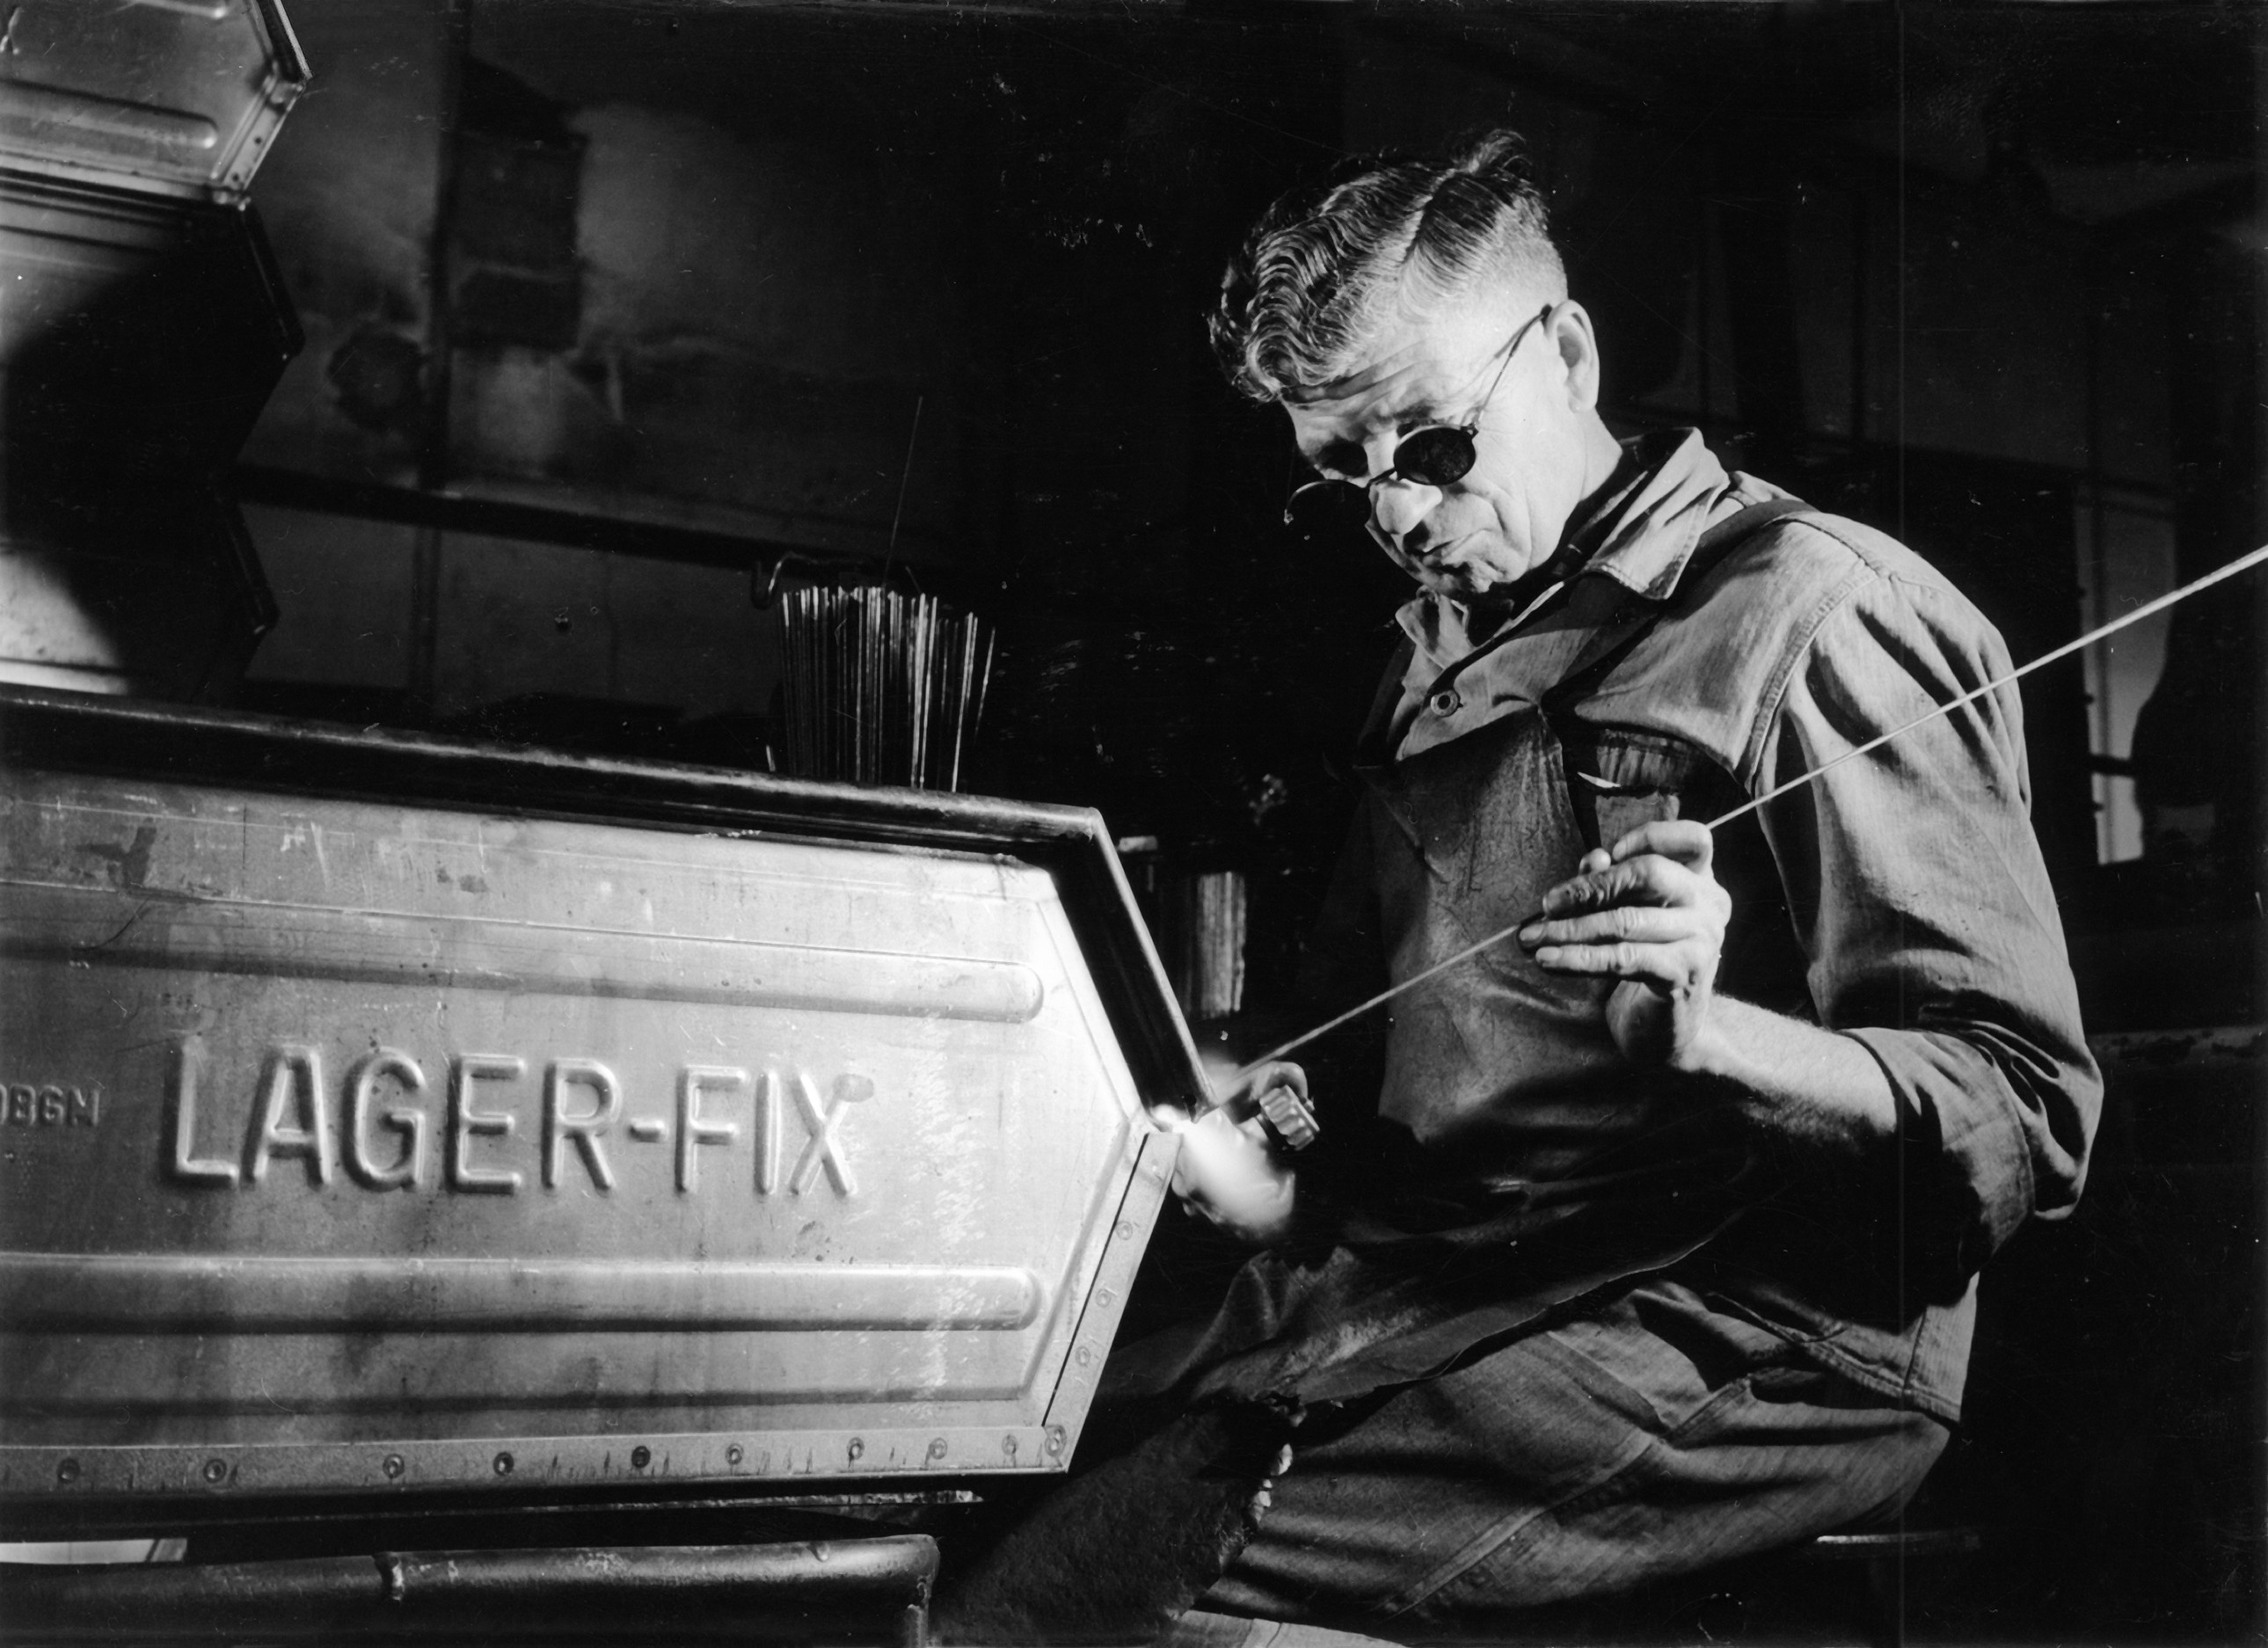
\includegraphics[width=0.48\textwidth]{images/lager_fix.jpg}
					\end{center}
					\vspace{-20pt}
					\caption{Lager fix}
					\vspace{-10pt}
				\end{wrapfigure}

	En 2008, le spécialiste logiciel, Salomon Automation, rejoint l'entreprise. Puis SSI SCHÄFER rachète l'entreprise danoise Handler A/S, expert en tours de stockage, en 2010. 2017 est un nouveau tournant pour l'entreprise avec la création de SSI SCHÄFER IT SOLUTIONS GMBH et une nouvelle dénomination sociale SSI SCHÄFER AUTOMATION GMBH.\\
			
	Vous pourrez par ailleurs trouver en annexe \ref{appendix:history} et \ref{appendix:map} une frise historique avec les dates importantes de l'histoire SSI SCHÄFER ainsi que la carte de toutes les filiales de l'entreprise.

			\subsubsection{SSI SCHÄFER en France}
	Le groupe SSI SCHÄFER est représenté par deux filiales en France, qui couvrent l'ensemble du territoire français et des besoins intralogistiques.\\

	Créée en 1963, SSI SCHAEFER SAS a son siège en historique en Moselle, on y retrouve notamment toutes les fonctions administratives et de soutien stratégique ainsi que la conception. Les commerciaux et techniciens de maintenance sont déployés sur l'ensemble du territoire français, ce qui garantit une proximité avec les clients et des temps de réaction brefs dans toute la France.\\

	En automne 2017, SSI SCHÄFER fait l'acquisition de GRN Logistic, basé à Cholet, qui vient compléter, de par son expertise dans le domaine des logiciels logistiques, l'expérience nationale et internationale du groupe dans la vente de solutions intralogistiques. Ce qui vient améliorer la compétence globale de SSI SCHÄFER en France.
			
		\subsubsection{Solutions intralogistiques}
	SSI SCHÄFER élabore, conçoit et fabrique des systèmes intralogistiques modulaires, destinés à tous les besoins en stockage, préparation de commandes et convoyage :
				\begin{itemize}
					\bdot{Solutions de stockage}
						\begin{itemize}
							\bdotoutlined{Rayonnage tous types}
							\bdotoutlined{Bacs et conteneurs}
							\bdotoutlined{Tours de stockage}
							\bdotoutlined{Trans-stockeurs}
							\bdotoutlined{Navettes}
							\bdotoutlined{Orbiters}
						\end{itemize}
					\bdot{Solutions de convoyage}
						\begin{itemize}
							\bdotoutlined{Convoyeur de bacs, cartons, palettes et plateaux}
							\bdotoutlined{Convoyeur aérien}
							\bdotoutlined{Système de transport sans conducteurs (AGVs)}
						\end{itemize}
					\bdot{Systèmes de préparation de commandes}
						\begin{itemize}
							\bdotoutlined{"Man to products" : pick by light, pick by voice, RF picking}
							\bdotoutlined{"Products to Man": caroussel, trieur, A-Frame, pick to tote}
							\bdotoutlined{Tours de stockage et rayonnages dynamiques}
						\end{itemize}
					\bdot{Solutions clefs en main}
						\begin{itemize}
							\bdotoutlined{Planification logistique globale et conseil}
							\bdotoutlined{Construction des bâtiments et installations}
							\bdotoutlined{Prestations de service et de maintenance sur mesure}
						\end{itemize}
				\end{itemize}

			\begin{figure}[h!]
				\begin{center}
					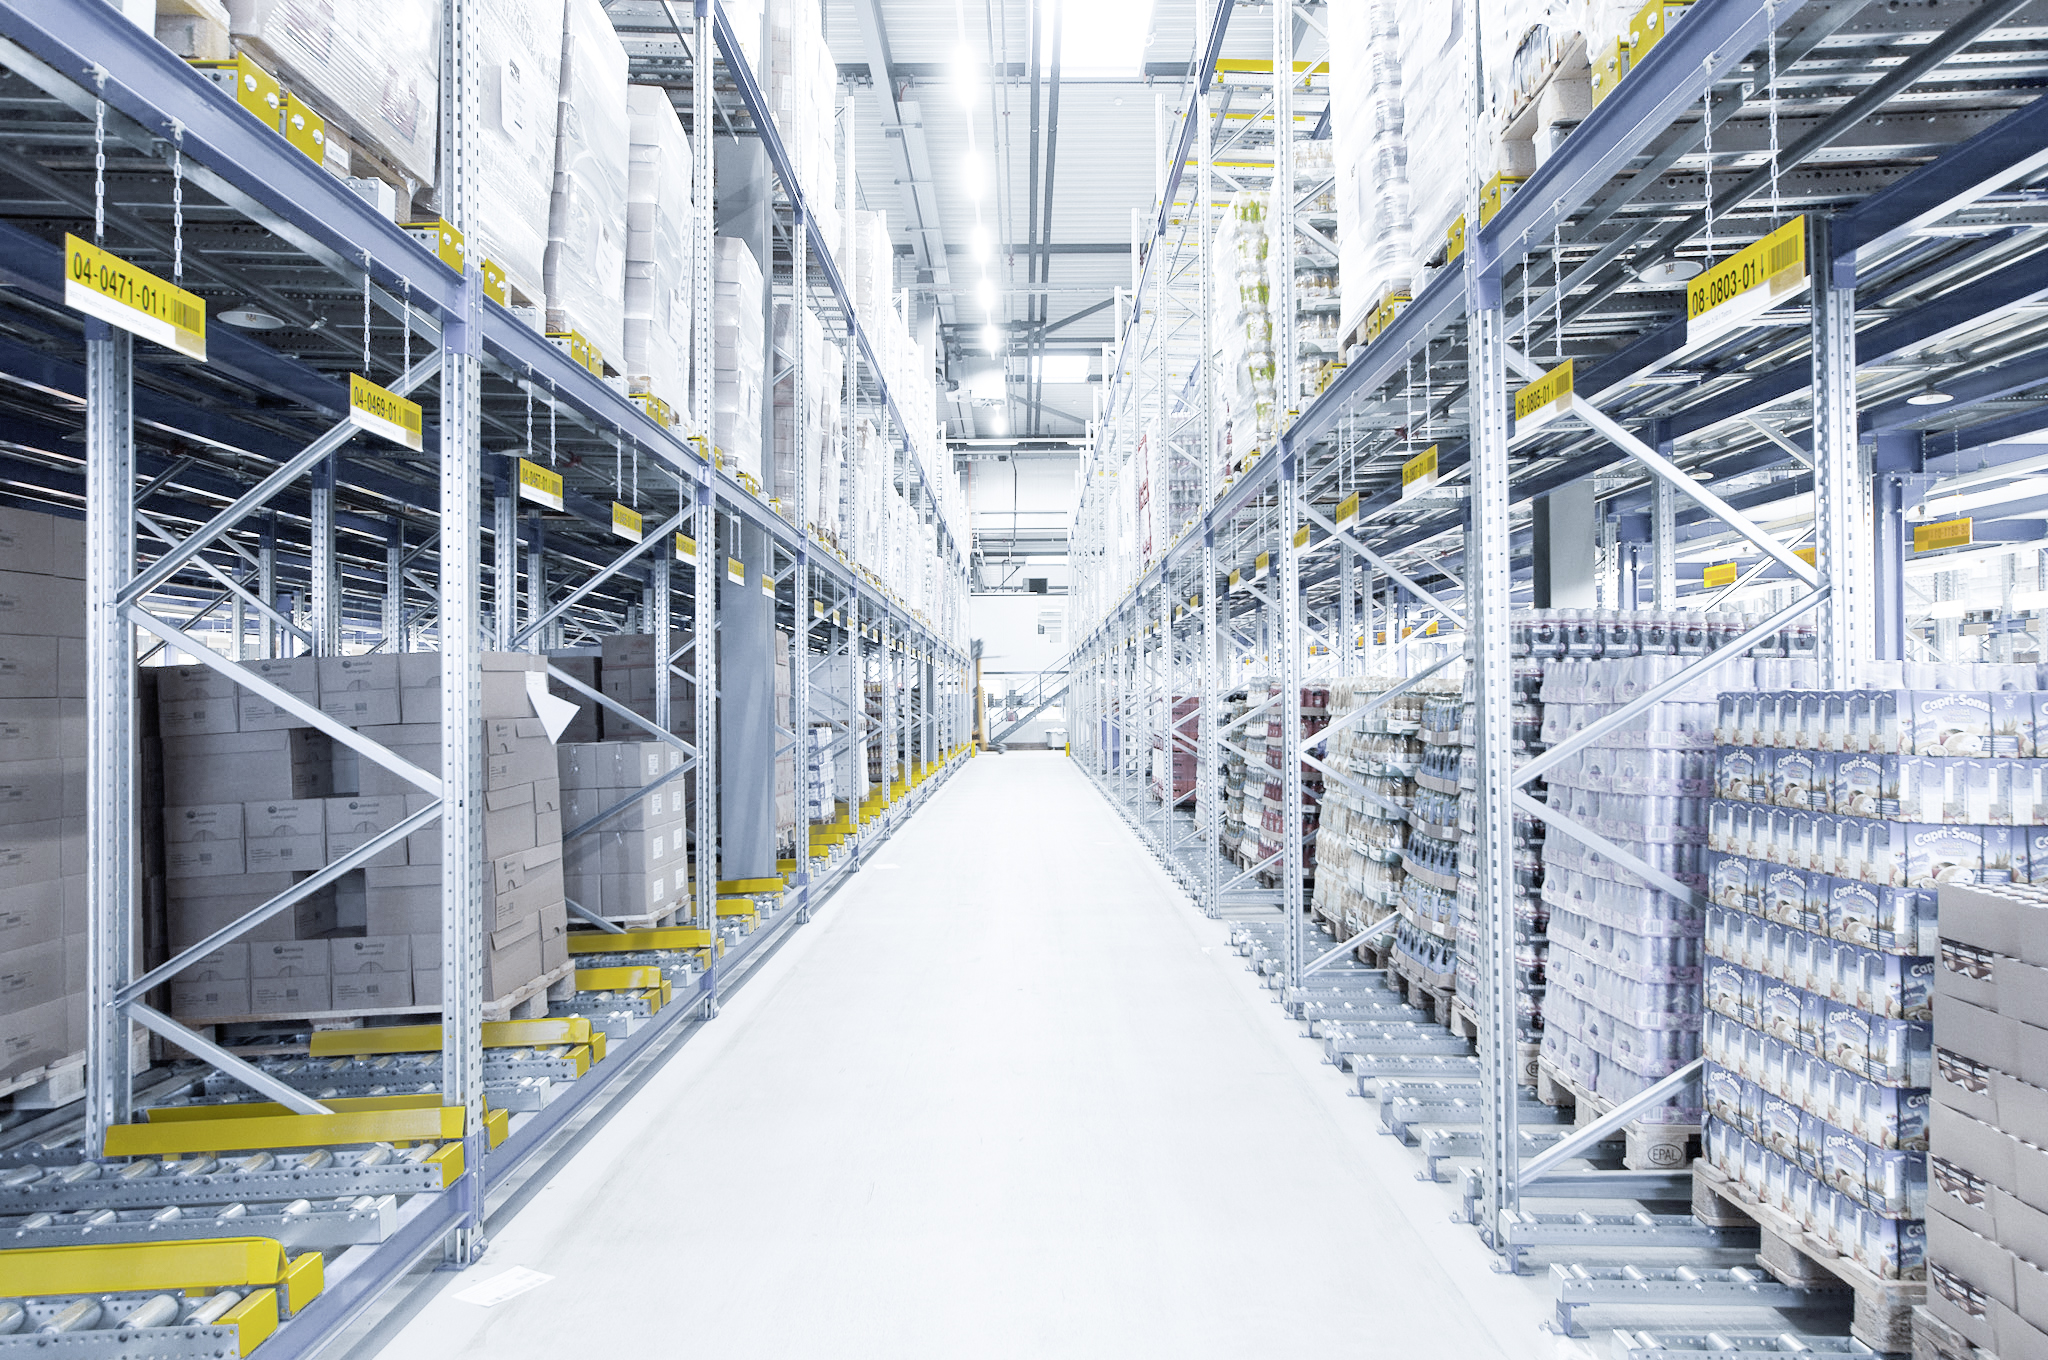
\includegraphics[width=0.7\linewidth]{images/intralogistic.jpg}
				\end{center}
				\caption{Exemple de solution intralogistique}
				\label{fig:intralogistic}
			\end{figure}	
	
			\subsubsection{Solutions logicielles}
	Les processus intralogistiques sont de plus en plus complexes. Dans les entrepôts manuels, automatisés et entièrement automatisés, d'innombrables processus doivent être contrôlés, visualisés et optimisés. Cela exige de l'expertise. En tant que premier fournisseur mondial de systèmes logistiques, SSI SCHÄFER ne se contente pas de proposer tout ce dont on a besoin pour des entrepôts, mais propose également l'expertise informatique.\\

				\noindent
				Exemples de logiciels logistiques développés par SSI SCHÄFER :
				\begin{itemize}
					\bdot{WAMAS}
					\bdot{MORPHEUS}
				\end{itemize}
				\vspace{\baselineskip}
				\par Nous nous intéresserons ici à MORPHEUS, logiciel développé en France par GRN Logistics, avec lequel j'ai travaillé durant mon stage.
		\subsection{MORPHEUS}
	La suite logicielle MORPHEUS est une gamme de logiciels dédiée à la gestion et à l'optimisation de la performance de la logistique. Elle est composée de différents modules :
			\begin{itemize}
				\bdot{\index{\gls{WMS}}Gestion des entrepôts}
				\bdot{\index{\gls{WCS}}Pilotage de stockeurs et de préparation de commandes automatisés}
			\end{itemize}
			\subsubsection{Morpheus \acrshort{wms}}
				\noindent				
				Les objectifs du WMS :%paragraph ?
				\begin{itemize}
					\bdot{Augmenter votre productivité}
					\bdot{Réduire les stocks}
					\bdot{Optimiser les surfaces de stockages}
					\bdot{Diminuer les erreurs}
				\end{itemize}
				\vspace{\baselineskip}
				Quelques fonctionnalités du WMS :
				\begin{itemize}
					\bdot{Moteur de règles pour la gestion des stratégies métiers}
					\bdot{Planification et pré-réception}
					\bdot{Création et affectation automatique des emplacements}
					\bdot{Ordonnancement manuel et automatique}
					\bdot{Pilotage des ressources humaines}
				\end{itemize}
			\subsubsection{Morpheus \acrshort{wcs}}
				\noindent
				Les objectifs du WCS :
				\begin{itemize}
					\bdot{Mécaniser et automatiser les flux}
					\bdot{Intégrer et synchroniser les WMS \& WCS}
					\bdot{Séquencez l'activité des équipements}
					\bdot{Superviser et optimiser les process}
				\end{itemize}
				\vspace{\baselineskip}
				Quelques fonctionnalités du WCS :
				\begin{itemize}
					\bdot{Pilotage de convoyeurs pour le transport de cartons, bacs...}
					\bdot{Pilotage du stockage et de la préparation de commandes}
					\bdot{Pilotage des trieurs / robots / meubles de tri}
				\end{itemize}
				\vspace{\baselineskip}
			Retrouvez plus d'informations sur le WMS et le WCS en annexe \ref{appendix:morpheusWMSFonctionnalites} et \ref{appendix:morpheusWCSFonctionnalites}

	\section{Cadre théorique}
			

	\section{Plan de recherche}

	\section{Présentation du projet réalisé au cours du stage}%en allemenand
		Introduction de la section

		\subsection{Application existante et projet}%mettre en annexe présentation delphi..
	À l'heure actuelle, Morpheus est une suite de logiciels regroupés au sein d'un client lourd développé en delphi. Cela implique que si vous voulons utiliser Morpheus, nous devons l'installer sur la machine sur laquelle nous en avons besoin ce qui peut-être parfois contraignant, surtout lorsque l'on a que des opérations de gestion à faire. Ainsi afin de simplifier l'accès à Morpheus, et ce sans avoir à installer de client lourd, il a été décidé de développer une application web qui permettra d'accéder à Morpheus depuis n'importe quel poste ayant un navigateur internet. Par ailleurs, en parallèle du projet de développer une version web du client Morpheus, un projet de refonte du client lourd a aussi été lancé. Ainsi dans le développement de l'application web je vais pouvoir à la fois m'inspirer de la version existante du client lourd ainsi qu'échanger avec le développeur en charge de la refonte du client lourd pour que nous puissions nous accorder sur certains points graphiques de l'interface utilisateur.


%mettre quelques captures d'écran de morpheus actuel..
	%Parler du client lourd morpheus + refonte client lourd..
		%développé en delphi, un peu vieux..

		\subsection{Architecture de l'application}
			schéma de l'architecture de l'application

		\subsection{Système de gestion de bases de données (SGBD)}
			Le système de gestion de bases de données utilisé par Morpheus est MSSqlServer développé par Microsoft. On peut notamment accéder aux bases de données via l'outil Microsoft SQL Server Management Studio.
			Actuellement beaucoup d'informations utiles à Morpheus sont stockés dans une base de données, et pas seulement les données affichées aux utilisateurs mais aussi de nombreux paramètres de gestion des interfaces graphiques. Il existe aussi de nombreuses procédures stockées permettant d'effectuer certaines actions. À l'heure actuelle, nous ne souhaitons pas changer ce système, c'est ainsi qu'afin de pouvoir accéder aux informations contenues dans la base de données, nous avons décidé de mettre en place une API REST servant de solution back-end à l'application web. Néanmoins si nous nous rendons compte que l'adaptation ou la création de nouvelles tables permettent l'amélioration de l'application web, nous ferons les ajustements nécessaires.

		\subsection{Back-end}
			
			
		\subsection{Front-end}
			L'application front-end de l'application web Morpheus est sans doute la plus importante du projet. En effet, elle représente la partie interface graphique et sera donc celle avec laquelle l'utilisateur va interagir besoin
	
			\subsubsection{Solutions possibles}
				Trois principales solutions ont été envisagées pour convenir aux objectifs de ce projet. Nous allons voir quelles sont ces solutions et pourquoi elles ont été envisagés.
				\paragraph{Delphi et TMS Software\\}%en annexe brève présentation de delphi et tms software + lien vers site ...
					Delphi et TMS Software ont été la première solution envisagée dans ce projet. En effet le langage delphi étant déjà utilisé au sein de l'entreprise SSI Schäfer, il a été logique pour eux de me proposer de réaliser le projet en utilisant cet outil. Néanmoins, nous nous sommes très vite rendu compte que cela n'allait pas être l'outil le plus adapté pour notre projet d'application web.\\
					%déjà utilisé par l'entreprise..
				\paragraph{Javascript\\}%en annexe brève présentation de javascript
					%JS vanilla
				\paragraph{ReactJS et devextreme\\}%en annexe brève présentation de reactjs et devextreme
					%React JS + devextreme..
		
			\subsubsection{Solution retenue}
				%ReactJS .. + pourquoi
				La solution que nous avons décidé de retenir est ReactJS, en effet cette technologie est celle qui correspond le mieux à ce que nous souhaitons faire dans le cadre de ce projet.

	\section{Specifications of the project}%en anglais Cahier des charges
		\subsection{Context}
			Here is s small summary of the context of the project, the launch of this project originated from the desire to develop a new Morpheus client with a new design and that is compatible with web technologies.

		\subsection{Goals}
			The goals of the project are 
			\begin{itemize}
				\bdot{Develop a morpheus client in full HTML 5 and responsive for some windows of the existing Mopheus client}
				\bdot{Experiment the development tools of TMS Web}
				\bdot{Make a UI mockup}
					\begin{itemize}
						\bdotoutlined{Main window}
							\begin{itemize}
								\bsquare{Menu}
									\begin{itemize}
										\bsquareoutlined{Icons}
										\bsquareoutlined{Style (as windows' style : colors)}
										\bsquareoutlined{X configurable levels and sub levels}
											\begin{itemize}
												\bdiamond{From a database : display or not some menu entries}
											\end{itemize}
									\end{itemize}
								\bsquare{Function buttons}
									\begin{itemize}
										\bsquareoutlined{Style}
										\bsquareoutlined{Icons}
										\bsquareoutlined{Size of buttons (16, 32 or 48)}
										\bsquareoutlined{Make buttons visible or not}
										\bsquareoutlined{Buttons layout depending of the number : alignements..}
									\end{itemize}
								\bsquare{Treeview}
									\begin{itemize}
										\bsquareoutlined{Style}
										\bsquareoutlined{Icons (in front of the label with touching triangle)}
										\bsquareoutlined{Display a list over a level following a request}
										\bsquareoutlined{Dynamically load of trees}
											\begin{itemize}
												\bdiamond{Configuration to make the trees visible or not}
											\end{itemize}
									\end{itemize}
							\end{itemize}
						\bdotoutlined{Style management}
						\bdotoutlined{MDI multi-window management (tabs)}
							\begin{itemize}
								\bsquare{Icons}
								\bsquare{Can be closed or not with a cross}
							\end{itemize}
						\bdotoutlined{Modal window management}
							\begin{itemize}
								\bsquare{Cross to close the window visible or not}
								\bsquare{Position memory}
							\end{itemize}
						\bdotoutlined{Login}
						\bdotoutlined{Database connection}
					\end{itemize}
				\bdot{Write a description of the client's operating mode at the ergonomic level}
				\bdot{Develop a first version with basic windows}
					\begin{itemize}
						\bdotoutlined{Main window}
							\begin{itemize}
								\bsquare{Menu}
									\begin{itemize}
										\bsquareoutlined{Icons}
										\bsquareoutlined{Style (as windows' style : colors)}
										\bsquareoutlined{X configurable levels and sub levels}
											\begin{itemize}
												\bdiamond{From a database : display or not some menu entries}
											\end{itemize}
									\end{itemize}
								\bsquare{Function buttons}
									\begin{itemize}
										\bsquareoutlined{Style}
										\bsquareoutlined{Icons}
										\bsquareoutlined{Size of buttons (16, 32 or 48)}
										\bsquareoutlined{Make buttons visible or not}
										\bsquareoutlined{Buttons layout depending of the number : alignements..}
									\end{itemize}
								\bsquare{Treeview}
									\begin{itemize}
										\bsquareoutlined{Style}
										\bsquareoutlined{Icons (in front of the label with touching triangle)}
										\bsquareoutlined{Display a list over a level following a request}
										\bsquareoutlined{Dynamically load of trees}
											\begin{itemize}
												\bdiamond{Configuration to make the trees visible or not}
											\end{itemize}
									\end{itemize}
							\end{itemize}
						\bdotoutlined{Style management}
						\bdotoutlined{MDI multi-window management (tabs)}
							\begin{itemize}
								\bsquare{Icons}
								\bsquare{Can be closed or not with a cross}
							\end{itemize}
						\bdotoutlined{Modal window management}
							\begin{itemize}
								\bsquare{Cross to close the window visible or not}
								\bsquare{Position memory}
							\end{itemize}
						\bdotoutlined{Login}
						\bdotoutlined{Database connection}
						\bdotoutlined{Access rights management}
						\bdotoutlined{Windows configuration management in xml}
							\begin{itemize}
								\bsquare{Window type}
								\bsquare{Associated grid}
								\bsquare{SQL query}
							\end{itemize}
					\end{itemize}
			\end{itemize}
		\subsection{Scope}
			The limits of the project are
			\begin{itemize}
				\bdot{Study of TMS components for development in Delphi X10, 2 HTML5 pages}
				\bdot{Construction of a new project for a new Morpheus client}
				\bdot{Definition of a new graphical interface}
				\bdot{Study of a graphical configuration mode by the end user}
				\bdot{Development of a UI mockup}
				\bdot{Development of HTML 5 technology under Delphi X10 in Pascal and generation and reading XML file}
				\bdot{Integration of a REST server driving in JSON}
			\end{itemize}
		\subsection{Targets}
			End users are morpheus users. They are therefore logistics technicians who work in warehouses.
		\subsection{Budget}	
			The project budget is made up of the following :
			\begin{itemize}
				\bdot{Investment of tms software tools: 1800€}
				\bdot{25 weeks * 5 days * 750€: budget time spent on development}
				\bdot{7 weeks * 1 day * 950€: budget time spent in management}
			\end{itemize}
		\subsection{Schedule}
			Project stages
			\begin{itemize}
				\bdot{Installation and configuration of tools}
				\bdot{Experimentation of tools}
				\bdot{Detailed writing of requirements}
				\bdot{Development of the new html5 client}
				\bdot{Testing and acceptance of the new customer}
				\bdot{Delivery}
			\end{itemize}
	
	%\section{Planning du projet}%+diagramme gantt..

	%\section{Objectifs du projet}
	
	\section{Aspect financier}
		dans le cas de morpheus le passage à un client web n'a pas un objectif financier néanmoins on peut supposer que dans d'autres cas il y aurait une envie de faire plus de profits, revendre un logiciel, passer moins de temps à installer et configurer.. mais pour les clients..	

		\subsection{Coûts}

		\subsection{Apports}


	\section{Aspect stratégique}

	\section{Aspect humain}


	\section{Partie scientifique}


	\section{Conclusion}


	\newpage
	
	\phantomsection

	%\renewcommand{\bibname}{Bibliographie}
	%\addto{\captionsfrench}{\renewcommand{\bibname}{Bibliographie}}
	\renewcommand\refname{Bibliographie}
	%site internet morpheus à changer dire que les pages ne sont plus d'actualités...
	\bibliography{testbib}
	\bibliographystyle{apalike}
	\addcontentsline{toc}{section}{Bibliographie}
	%\addcontentsline{toc}{section}{\bibliographyname}

	%\newpage

	\phantomsection
	\printindex

	\newpage

	\phantomsection
	\appendix% On passe aux annexes
	\section*{Annexes}
	\addcontentsline{toc}{section}{Annexes}
		%si moins de 26 annexes
		\renewcommand{\thesubsection}{\Alph{subsection}}
		\counterwithin{figure}{subsection}
		\counterwithin{table}{subsection}
		%sinon
		%\renewcommand{\thesubsection}{\Roman{subsection}}

		\subsection{Dates importantes de l'histoire SSI SCHÄFER}\label{appendix:history}
			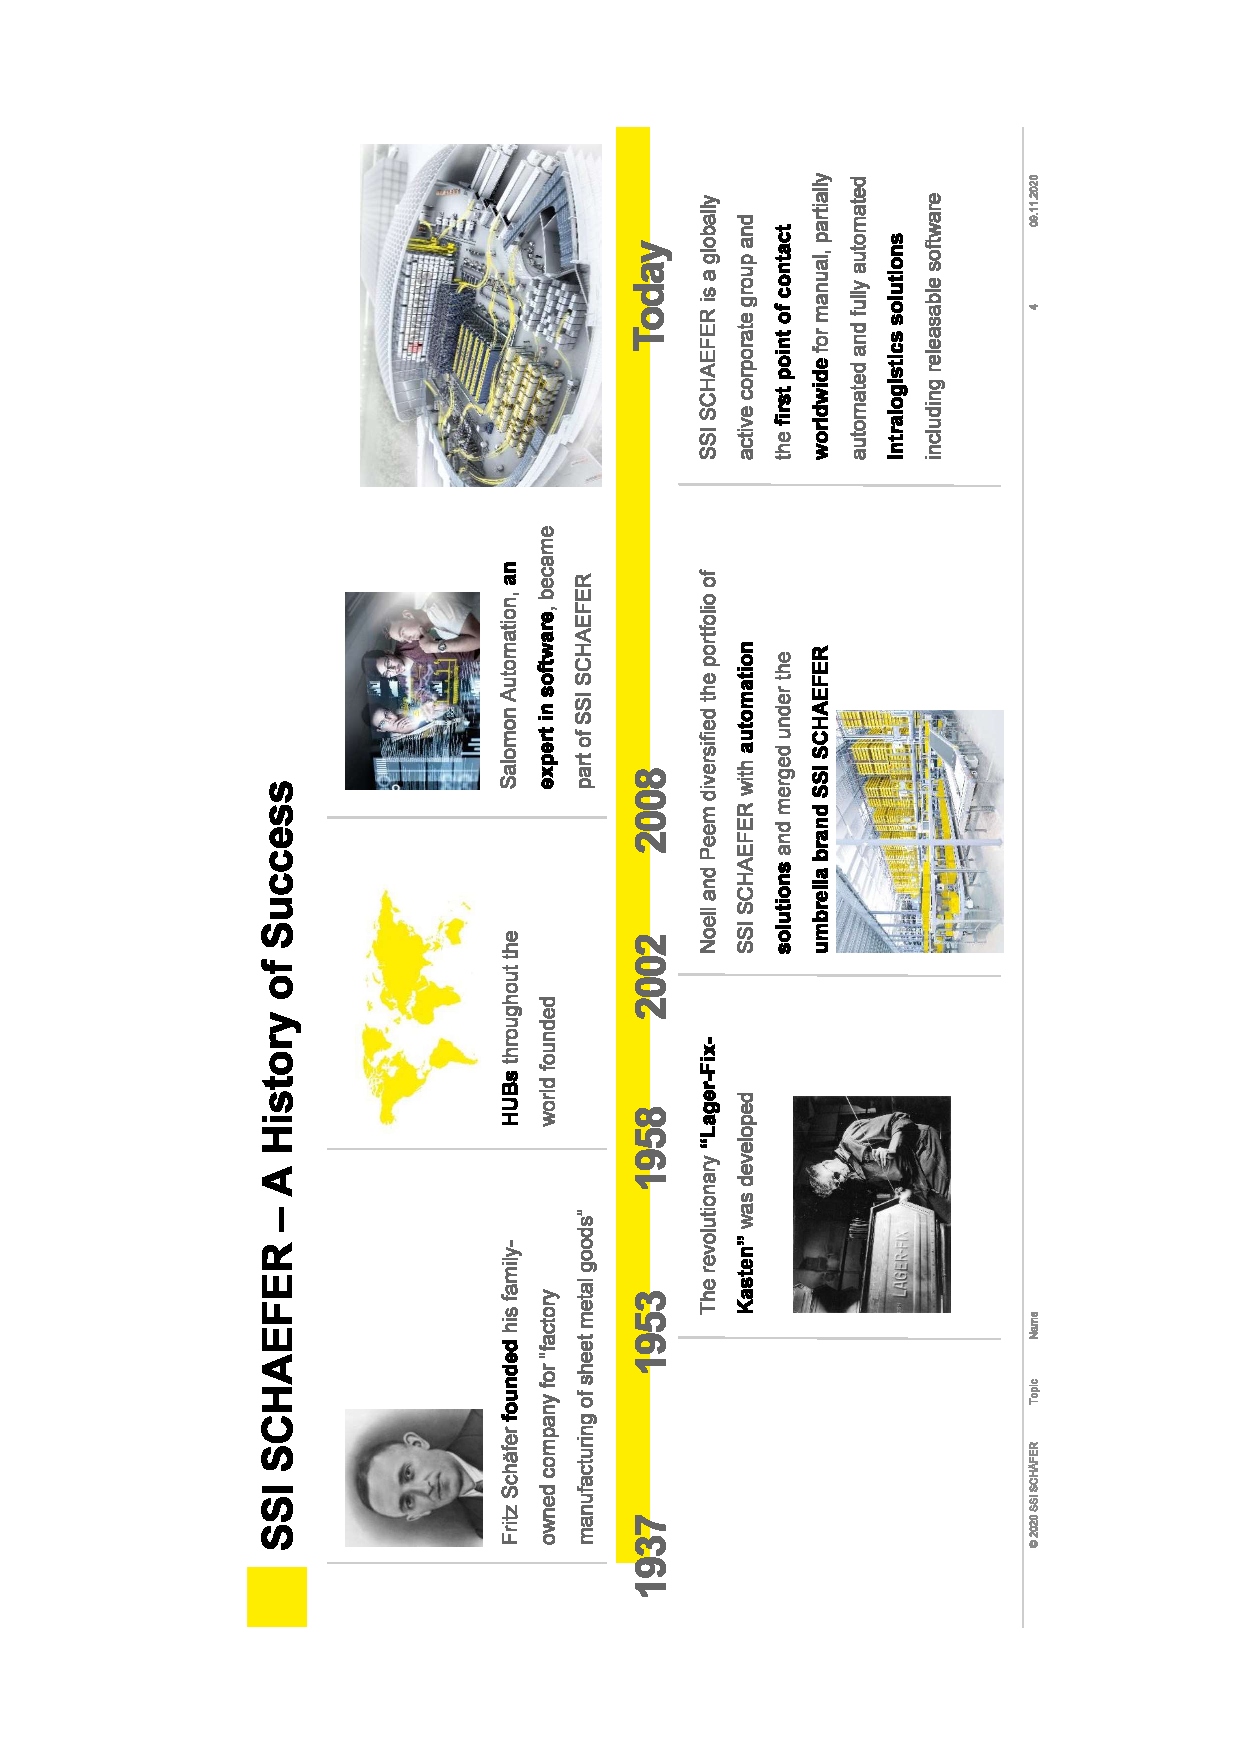
\includegraphics[width=0.8\linewidth]{images/history.pdf}

		\newpage
		\subsection{Carte des filiales SSI SCHÄFER}\label{appendix:map}
			%\includegraphics[width=0.8\textwidth]{tikzpgf.pdf}
			\begin{center}
				\includegraphics[width=\textwidth]{images/world_map.jpg}
			\end{center}
				%\includegraphics[width=\textwidth]{world_map.jpg}
		\newpage


		\subsection{Liste complète des fonctionnalités de MORPHEUS WMS}\label{appendix:morpheusWMSFonctionnalites}
			\begin{figure}[h!]
					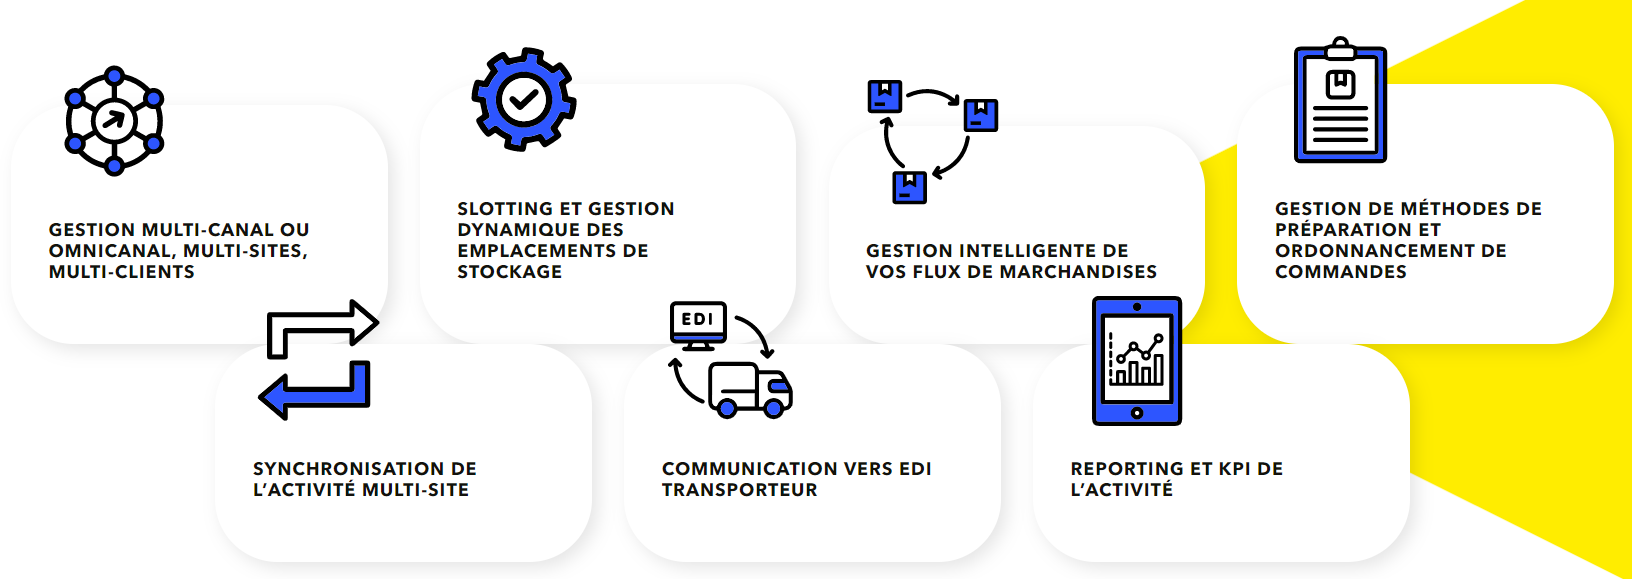
\includegraphics[width=\linewidth]{images/morpheus_wms_fonctionnalites.png}
					\caption{Fonctionnalités de Morpheus WMS}%\cite{screenshot}
					\label{fig:morpheus_wms_fonctionnalites}
			\end{figure}
		\subsection{Liste complète des fonctionnalités de MORPHEUS WCS}\label{appendix:morpheusWCSFonctionnalites}
			\begin{figure}[h!]
					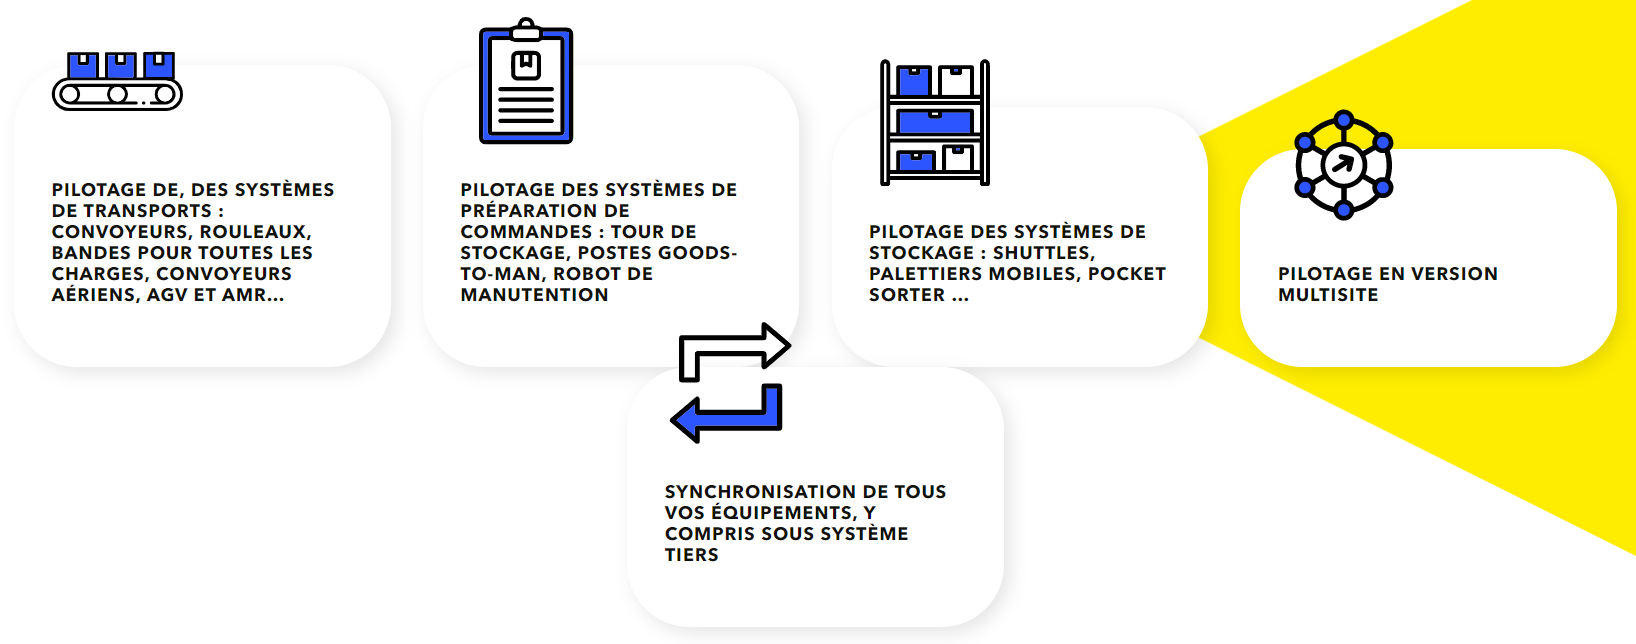
\includegraphics[width=\linewidth]{images/morpheus_wcs_fonctionnalites.png}
					\caption{Fonctionnalités de Morpheus WCS}%\cite{screenshot}
					\label{fig:morpheus_wcs_fonctionnalites}
			\end{figure}

		\newpage

	\section*{Mots clés}
	Liste des mots clés : delphi, développement, développement informatique, logistique, France, Cholet, WMS, WCS, MORPHEUS, tms, react, nodejs, devexpress, devextreme
	%en anglais
	%en allemand
	\newpage

	\phantomsection
	\section*{Résumés}
	\addcontentsline{toc}{section}{Résumés}
		\subsection*{Résumé}
		\addcontentsline{toc}{subsection}{Résumé}

		\subsection*{Summary}
		\addcontentsline{toc}{subsection}{Summary}


		\subsection*{Zusammenfassung}
		\addcontentsline{toc}{subsection}{Zusammenfassung}


	
		\newpage
\end{document}